\documentclass[runningheads]{CMSIM}
\usepackage[T1]{fontenc}
\usepackage{amsmath}
\usepackage{amssymb}
\usepackage{graphicx}
\usepackage[space]{cite}
\usepackage[english]{babel}


\pagestyle{empty}
\renewcommand{\thefootnote}

\setlength{\headsep}{0pt}

\title*{A model of random walk with varying transition probabilities}

\titlerunning{\it R. W. with varying transition prob.}

\author{
    Tom\'{a}\v{s} Kou\v{r}im\inst{1}
    \and
    Petr Volf\inst{2}
}

\authorrunning{\it Kou\v{r}im and Volf}

\institute{
    Faculty of Nuclear Sciences and Physical Engineering, Czech Technical University in Prague,
    Czech Republic\\
    (E-mail: {\tt kourim@outlook.com})
    \and
    Institute of Information Theory and Automation, Academy of Sciences of the Czech Republic, Prague\\
    (E-mail: {\tt volf@utia.cas.cz})
}


\setcounter{page}{1}
\begin{document}
    \thispagestyle{empty}
    \maketitle
    \setlength{\leftskip}{0pt}
    \setlength{\headsep}{16pt}
    \footnote{\begin{tabular}{p{11.2cm}r}
                  \small {\it $6^{th}$SMTDA Conference Proceedings, 2--5 June 2020, Barcelona, Spain} \\
                  \small \textcopyright {} 2020 ISAST & 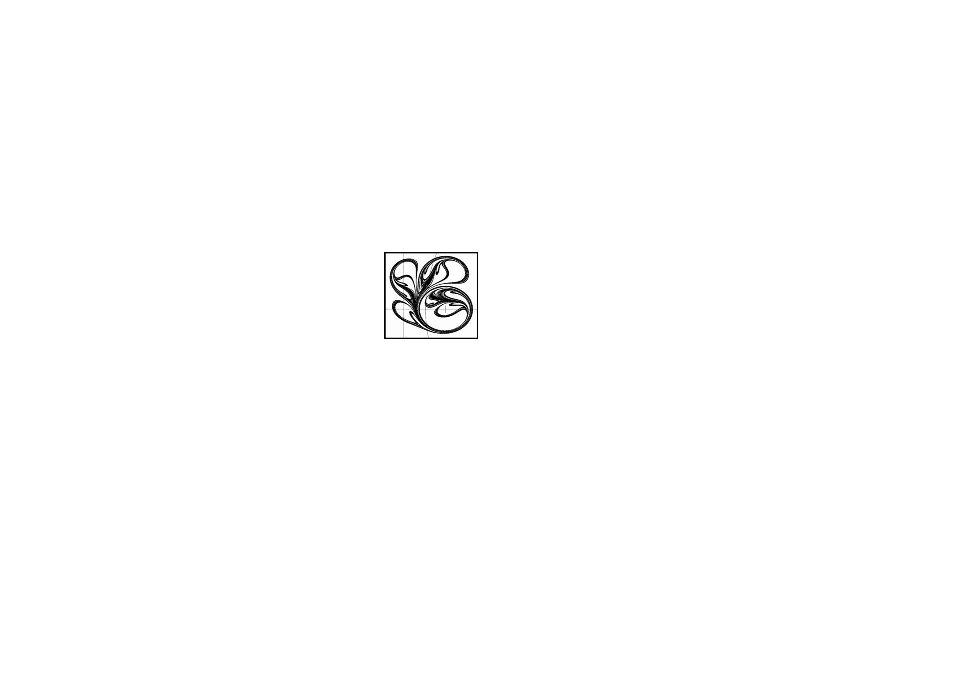
\includegraphics[scale=0.38]{CMSIM_Logo}
    \end{tabular}}
    \begin{abstract}
        This paper considers a model of one-dimensional discrete time
        random walk in which the position of the walker is controlled by
        varying transition probabilities.
        These probabilities depend
        explicitly on the previous move of the walker and implicitly on the
        entire walk history.
        Hence, transition probabilities evolve in time
        making the walk a non-Markovian stochastic process.
        The paper follows
        on the recent work of the authors.
        Two basic versions of the model
        are introduced, some of their properties are recalled and new theoretical
        results derived.
        Then, more complex variants of models are presented.
        Development of walks themselves as well as the properties of connected
        sequences of transition probabilities are illustrated also with the
        aid of simulations.
        Possible applications of the model in real life
        situations are discussed and briefly described, too.
        \keyword{Random walk, history dependent transition probabilities, success punishing/rewarding walk}
    \end{abstract}


    \section{Introduction}\label{sec:introduction}

    Stochastic processes and the corresponding mathematical theory represent
    a significant part of mathematics.
    One of the most prominent of such
    processes is the random walk, introduced by K. Pearson over hundred
    years ago~\cite{pearson1905problem}.
    This concept has been then further
    elaborated by many authors creating a number of different versions
    of a random walk~\cite{spitzer2013principles} and there are still
    new possibilities and options how the classical random walk can be
    altered and adapted to specific application field.
    The model discussed
    in this paper follows on the work of Turban~\cite{turban2010random}
    and represents yet another version of a random walk, walk with varying
    transition probabilities.
    The model falls within a rather broad class
    of processes presented in recent work of Davis and Liu~\cite{davis2012theory}, but not all assumptions from~\cite{davis2012theory} are met.

    The original inspiration for the model comes from one of its applications -- modelling of sports events.
    Many types of sport, such as tennis
    or volleyball, are played in a strictly discrete matter with steps
    divided by individual \emph{points},\emph{ games }or \emph{sets}.
    One sport match can be thus viewed as a random walk with individual
    parts of the match representing the steps of the walk.
    Success, i.e.\ scoring a point or winning a set, then significantly affects further
    development of the entire walk by changing the transition probability.
    Other real life situations with similar properties can be found everywhere
    in areas where both ``successes'' or ``failures'' occur.
    In fact,
    also discrete time recurrent counts data occurrence can be often modelled
    in a similar way, when the event probability is affected by the process
    recent history.
    Such cases include the recurrence of diseases, recidivism
    in crime or repeated defects and maintenance of a technical
    device.

    The present contribution continues on the recent authors' exploration
    of the model of random walk with varying probabilities.
    Selected
    properties of the model are presented and possible real life implementations
    of the model are discussed.
    The rest of the paper is organized as
    follows.
    Next section introduces theoretical properties of the model
    and describes in detail the two main variants of the model.
    Section \ref{sec:Model-application}
    presents possible applications of the model and the last section concludes
    this work.


    \section{Theoretical properties}\label{sec:theoretical-properties}

    As already mentioned, modelling sport events served as a motivation for the presented model.
    The probability of a success (i.e. scoring a goal, achieving
    a point etc.) is at the center of interest in such modelling.
    After each occurrence
    of such success this probability either decreases or increases, and
    thus two basic model alternatives exist -- \emph{success punishing} and \emph{success rewarding}.
    The basic version of the model operates
    with starting success probability $p_{0}$ and a memory coefficient
    $\lambda$ affecting the severity of probability change after a success
    as input parameters.
    Formally the walk is defined as follows:
    \begin{definition}
        \label{def:walk_definition}Let $\ensuremath{p_{0}\in(0,\,1),\,\lambda\in(0,\,1)}$
        be constant parameters, ${\{P_{n}\}}_{n=0}^{\infty}$ and ${\{X_{n}\}}_{n=1}^{\infty}$
        sequences of discrete random variables with $P_{0}=p_{0}$.
        For $t\ge1$ let
        \[
            P(X_{t}=1|P_{t-1}=p_{t-1})=p_{t-1},\,\,\,P(X_{t}=-1|P_{t-1}=p_{t-1})=1-p_{t-1},
        \]
        and (\emph{success punishing)}
        \begin{equation}
            P_{t}=\lambda P_{t-1}+\frac{1}{2}(1-\lambda)(1-X_{t})\label{eq:def_p_sp}
        \end{equation}
        or (\emph{success rewarding)
            \begin{equation}
                P_{t}=\lambda P_{t-1}+\frac{1}{2}(1-\lambda)(1+X_{t}).\label{eq:def_p_sr}
            \end{equation}
        }The sequence ${\{S_{n}\}}{}_{n=0}^{\infty},\;S_{N}=S_{0}+\sum_{i=1}^{N}X_{i}$
        for $n\in\mathbb{N}$, with $S_{0}\in\mathbb{R}$ some given starting
        position, is called a \emph{random walk with varying probabilities},
        with ${\{X_{n}\}}_{n=1}^{\infty}$ being the steps of the walker and
        ${\{P_{n}\}}_{n=0}^{\infty}$ transition probabilities.
        Depending
        on the chosen formula to calculate $P_{t}$ the walk type is either
        \emph{success punishing}~\eqref{eq:def_p_sp} or \emph{success rewarding}~\eqref{eq:def_p_sr}.
    \end{definition}

    The model was first introduced in~\cite{ja2017ddny} and a more thorough
    description was provided in~\cite{ja2019teze}.
    Selected properties
    were then presented in~\cite{ja2019apmat} and a practical implementation
    of the model in modelling tennis matches was presented in~\cite{ja2019mathsport_proc}.
    The basic results are recalled in the following sections and then
    variance of $S_{t}$ is derived and described in more detail.

    \subsection{Success punishing model}\label{subsec:success-punishing-model}

    The basic properties of the \emph{success punishing }version of the
    walk are presented in this section.
    Previous results are presented
    as a set of expressions only, the reader is kindly asked to see referred
    papers for full proves of those expressions.
    Newly described properties
    are then provided with full proves and all necessary details.

    For the expected value and variance of the step size for the $t\ge1$
    iteration of the walk $X_{t}$ it holds~\cite{ja2019apmat}
    \begin{equation}
        EX_{t}=(2\lambda-1)^{t-1}(2p_{0}-1),\label{eq:e_x_t_sp}
    \end{equation}
    \begin{equation}
        Var\,X_{t}=1-(2\lambda-1)^{2(t-1)}(2p_{0}-1)^{2}.\label{eq:var_x_t_sp}
    \end{equation}

    For the expected value and variance of the transition probability
    for the $t\ge1$ iteration of the walk $P_{t}$ it holds~\cite{ja2017ddny,ja2019apmat}
    \begin{equation}
        EP_{t}=(2\lambda-1)^{t}p_{0}+\frac{1-(2\lambda-1)^{t}}{2},\label{eq:e_p_t_sp}
    \end{equation}
    \begin{equation}
        Var\,P_{t}=(3\lambda^{2}-2\lambda)^{t}p_{0}^{2}+\sum_{i=0}^{t-1}K(i;p_{0},\lambda)(3\lambda^{2}-2\lambda)^{t-1-i}-k(t;p_{o},\lambda)^{2},\label{eq:var_p_t_sp}
    \end{equation}
    where
    \[
        k(t;p_{o},\lambda)^{2}=EP_{t}=(2\lambda-1)^{t}p_{0}+\frac{1-(2\lambda-1)^{t}}{2}
    \]
    and
    \[
        K(t;p_{o},\lambda)^{2}=k(t;p_{o},\lambda)^{2}\cdot(-3\lambda^{2}+4\lambda-1)+(1-\lambda)^{2}.
    \]

    Finally, the expected position of the walker $S_{t}$ after $t\geq1$
    iterations can be expressed as~\cite{ja2017ddny}
    \begin{equation}
        ES_{t}=S_{0}+(2p_{0}-1)\frac{1-(2\lambda-1)^{t}}{2(1-\lambda)}.\label{eq:e_s_t_sp}
    \end{equation}

    The last formula missing is the one expressing the variance of the
    position of the walker $Var\,S_{t}$.
    Before it is presented, let
    us first prove a support proposition.
    \begin{proposition}
        \label{prop:e_p_s_t_sp}
        For all $t\ge1$
        \begin{equation}
            E(P_{t}S_{t})=(2\lambda-1)^{t}p_{0}S_{0}+\sum_{i=0}^{t-1}(2\lambda-1)^{i}q(t-1-i;p_{0},S_{0},\lambda),\label{eq:e_p_s_t_sp}
        \end{equation}
        where
        \[
            q(j;p_{0},S_{0},\lambda)=(1-\lambda)s(j;p_{0},S_{0},\lambda)+2\lambda\pi(j;p_{0},\lambda)+(1-2\lambda)p(j;p_{0},\lambda)+\lambda-1
        \]
        and $p(j;p_{0},\lambda)=EP_{j}$ is given by~\eqref{eq:e_p_t_sp}, $s(j;p_{0},S_{0},\lambda)=ES_{j}$
        by~\eqref{eq:e_s_t_sp} and $\pi(j;p_{0},\lambda)=EP_{j}^{2}$
        is given as
        \begin{equation}
            EP_{t}^{2}=(3\lambda^{2}-2\lambda)^{t}p_{0}^{2}+\frac{1-(3\lambda^{2}-2\lambda)^{t}}{3\lambda+1}\frac{(\lambda+1)}{2}-(p_{0}-\frac{1}{2})(3\lambda^2 - 4\lambda +1)M(t-1;\lambda),\label{eq:e_p2_t_sp}
        \end{equation}
        where
        \[
            M(t;\lambda)=\sum_{i=0}^{t-1}(3\lambda^{2}-2\lambda)^{t-1-i}(2\lambda-1)^{i}.
        \]
    \end{proposition}

    \begin{proof}
        The formula for $EP_{t}^{2}$ follows from the proof of Proposition
        2.5 in~\cite{ja2019apmat}.
        To prove~\eqref{eq:e_p_s_t_sp} let us
        start with expressing the value of $E(P_{t}S_{t})$ from the knowledge
        of past steps as
        \begin{gather*}
            E(P_{t}S_{t})=E[E(P_{t}S_{t}|P_{t-1})]=\\
            =E[E((\lambda P_{t-1}+\frac{1}{2}(1-\lambda)(1-X_{t}))(S_{t-1}+X_{t})|P_{t-1})]=\\
            =E[E(\lambda P_{t-1}S_{t-1}+\frac{1-\lambda}{2}S_{t-1}-\frac{1-\lambda}{2}X_{t}S_{t-1}+\\
                +\lambda X_{t}P_{t-1}+\frac{1-\lambda}{2}X_{t}-\frac{1-\lambda}{2}X_{t}^{2}|P_{t-1})].\\
        \end{gather*}
        Using $E(X_{t}|P_{t-1})=2P_{t-1}-1$ and $EX_{t}^{2}=1$ we get
        \begin{equation}
            E(P_{t}S_{t})=(2\lambda-1)E(P_{t-1}S_{t-1})+(1-\lambda)ES_{t-1}+2\lambda EP_{t-1}^{2}+(2\lambda-1)EP_{t-1}+\lambda-1.\label{eq:e_p_s_t-1_t_sp}
        \end{equation}
        Further we will continue using mathematical induction.
        For $t=1$
        using the definition of the walk it holds that
        \begin{gather*}
            E(P_{1}S_{1})=p_{0}(p_{0}\lambda(S_{0}+1))+(1-p_{0})[(1-(1-p_{0})\lambda)(S_{0}-1)]=\\
            =(2\lambda-1)p_{0}S_{0}+(1-\lambda)S_{0}+2\lambda p_{0}^{2}-(2\lambda-1)p_{0}+\lambda-1.\\
        \end{gather*}
        When substituting $t=1$ into~\eqref{eq:e_p_s_t_sp} we obtain
        \begin{gather*}
            E(P_{1}S_{1})=(2\lambda-1)p_{0}S_{0}+\sum_{i=0}^{0}(2\lambda-1)^{i}q(0-i;p_{0},S_{0},\lambda)=\\
            =(2\lambda-1)p_{0}S_{0}+(1-\lambda)s(0;p_{0},\lambda)+\\
            +2\lambda\pi(0;p_{0},\lambda)+(1-2\lambda)p(0;p_{0},\lambda)+\lambda-1\\
        \end{gather*}
        and finally using~\eqref{eq:e_p_t_sp},~\eqref{eq:e_s_t_sp} and~\eqref{eq:e_p2_t_sp}
        \[
            E(P_{1}S_{1})=(2\lambda-1)p_{0}S_{0}+(1-\lambda)S_{0}+2\lambda p_{0}^{2}+(1-2\lambda)p_{0}+\lambda-1.
        \]
        Equation~\eqref{eq:e_p_s_t_sp} thus holds for $t=1$.
        Now for the
        induction step $t\rightarrow t+1$, after substituting \eqref{eq:e_p_s_t_sp}
        into \eqref{eq:e_p_s_t-1_t_sp} we get $E(P_{t+1}S_{t+1})=$
        \begin{gather*}
            =(2\lambda-1)E(P_{t}S_{t})+(1-\lambda)ES_{t}+2\lambda EP_{t}^{2}+(2\lambda-1)EP_{t}+\lambda-1=\\
            =(2\lambda-1)[(2\lambda-1)^{t}p_{0}S_{0}+\sum_{i=0}^{t-1}(2\lambda-1)^{i}q(t-1-i)]+(1-\lambda)s(t)+\\
            +2\lambda\pi(t)+(2\lambda-1)p(t)+\lambda-1=\\
            =(2\lambda-1)^{t+1}p_{0}S_{0}+\sum_{i=0}^{t}(2\lambda-1)^{i}q(t-i).\\
        \end{gather*}
    \end{proof}
    \begin{theorem}
        \label{thm:VarSt_sp}For all $t\ge1$
        \[
            Var\,S_{t}=t+4\sum_{i=0}^{t-1}\sigma(i;p_{0},0,\lambda)-a(t;p_{0},\lambda),
        \]
        with $\sigma(i;p_{0},S_{0},\lambda)=E(P_{t}S_{t})$ given by Proposition ~\ref{prop:e_p_s_t_sp}
        and
        \[
            a(t;p_{0},\lambda)=(2p_{0}-1)\sum_{i=0}^{t-1}\frac{1-(2\lambda-1)^{i}}{1-\lambda}+(2p_{0}-1)^{2}\frac{(1-(2\lambda-1)^{t})^{2}}{4(1-\lambda)^{2}}.
        \]
    \end{theorem}

    \begin{proof}
        As clearly the value $S_{0}$ does not affect the variance, let us
        from now assume $S_{0}=0$.
        From the definition of variance
        \begin{equation}
            Var\,S_{t}=ES_{t}^{2}-E^{2}S_{t}\label{eq:var_s_t_rozepsano_sp}
        \end{equation}
        and~\eqref{eq:e_s_t_sp} follows that to prove the proposition it
        is enough to prove that
        \begin{equation}
            ES_{t}^{2}=t+4\sum_{i=0}^{t-1}\sigma(i;p_{0},0,\lambda)-(2p_{0}-1)\sum_{i=0}^{t-1}\frac{1-(2\lambda-1)^{i}}{1-\lambda}.\label{eq:e_s2_t_sp}
        \end{equation}
        First of all, let us express $ES_{t}^{2}$ from the knowledge of past
        walk development.
        From the definition of the expected value and the
        definition of the walk it follows
        \begin{gather*}
            ES_{t}^{2}=E[E(S_{t}^{2}|P_{t-1})]=E[E((S_{t-1}+X_{t})^{2}|P_{t-1})]=\\
            =E(S_{t-1}^{2}+2(2P_{t-1}-1)S_{t-1}+1)=
        \end{gather*}
        \begin{equation}
            =ES_{t-1}^{2}+4E(P_{t-1}S_{t-1})-2ES_{t-1}+1,\label{eq:e_s2_t-1_t_sp}
        \end{equation}
        where the fact that $EX_{t}^{2}=1$ was used.
        The theorem will be proved using mathematical induction again.
        For $t=1$ we get from the definition of the walk
        \[
            ES_{1}^{2}=p_{0}(S_{0}+1)^{2}+(1-p_{0})(S_{0}-1)^{2}=1.
        \]
        Substituting $t=1$ into~\eqref{eq:e_s2_t_sp} we obtain
        \[
            ES_{1}^{2}=1+4\sigma(0;p_{0},0,\lambda)-(2p_{0}-1)\frac{1-(2\lambda-1)^{0}}{1-\lambda}=1
        \]
        and~\eqref{eq:e_s2_t_sp} thus holds for $t=1$.
        Now for the induction
        step $t\rightarrow t+1$ we get by substituting~\eqref{eq:e_s2_t_sp}
        into (\ref{eq:e_s2_t-1_t_sp})
        \begin{gather*}
            ES_{t+1}^{2}=ES_{t}^{2}+4E(P_{t}S_{t})-2ES_{t}+1=\\
            =t+4\sum_{i=0}^{t-1}\sigma(i;p_{0},0,\lambda)-(2p_{0}-1)\sum_{i=0}^{t-1}\frac{1-(2\lambda-1)^{i}}{1-\lambda}+\\
            +4\sigma(t;p_{0},0,\lambda)-2(2p_{0}-1)\frac{1-(2\lambda-1)^{t}}{2(1-\lambda)}+1=\\
            (t+1)+4\sum_{i=0}^{t}\sigma(i;p_{0},0,\lambda)-(2p_{0}-1)\sum_{i=0}^{t}\frac{1-(2\lambda-1)^{i}}{1-\lambda},\\
        \end{gather*}
        which proves~\eqref{eq:e_s2_t_sp}.
        Substituting~\eqref{eq:e_s2_t_sp}
        and~\eqref{eq:e_s_t_sp} into~\eqref{eq:var_s_t_rozepsano_sp} then
        proves the theorem.
    \end{proof}
    \begin{corollary}
        \label{cor:var_s_t_sp}For $t\rightarrow+\infty$
        \[
            Var\,S_{t}=+\infty
        \]
        and
        \[
            \lim_{t\rightarrow+\infty}(Var\,S_{t}-(c_{1}(p_{0},\lambda)t+c_{2}(p_{0},\lambda))=0,
        \]
        where $c_{i}(p_{0},\lambda)$ are some $t$-independent constants.
    \end{corollary}

    Corollary~\ref{cor:var_s_t_sp} shows that with $t\rightarrow+\infty$
    $Var\,S_{t}$ behaves as a linear function with respect to $t$.
    This
    can be seen also on Figure~\ref{fig:var_s_t_sp} together with a
    comparison of observed and theoretical values of $Var\,S_{t}$.

    \begin{figure}
        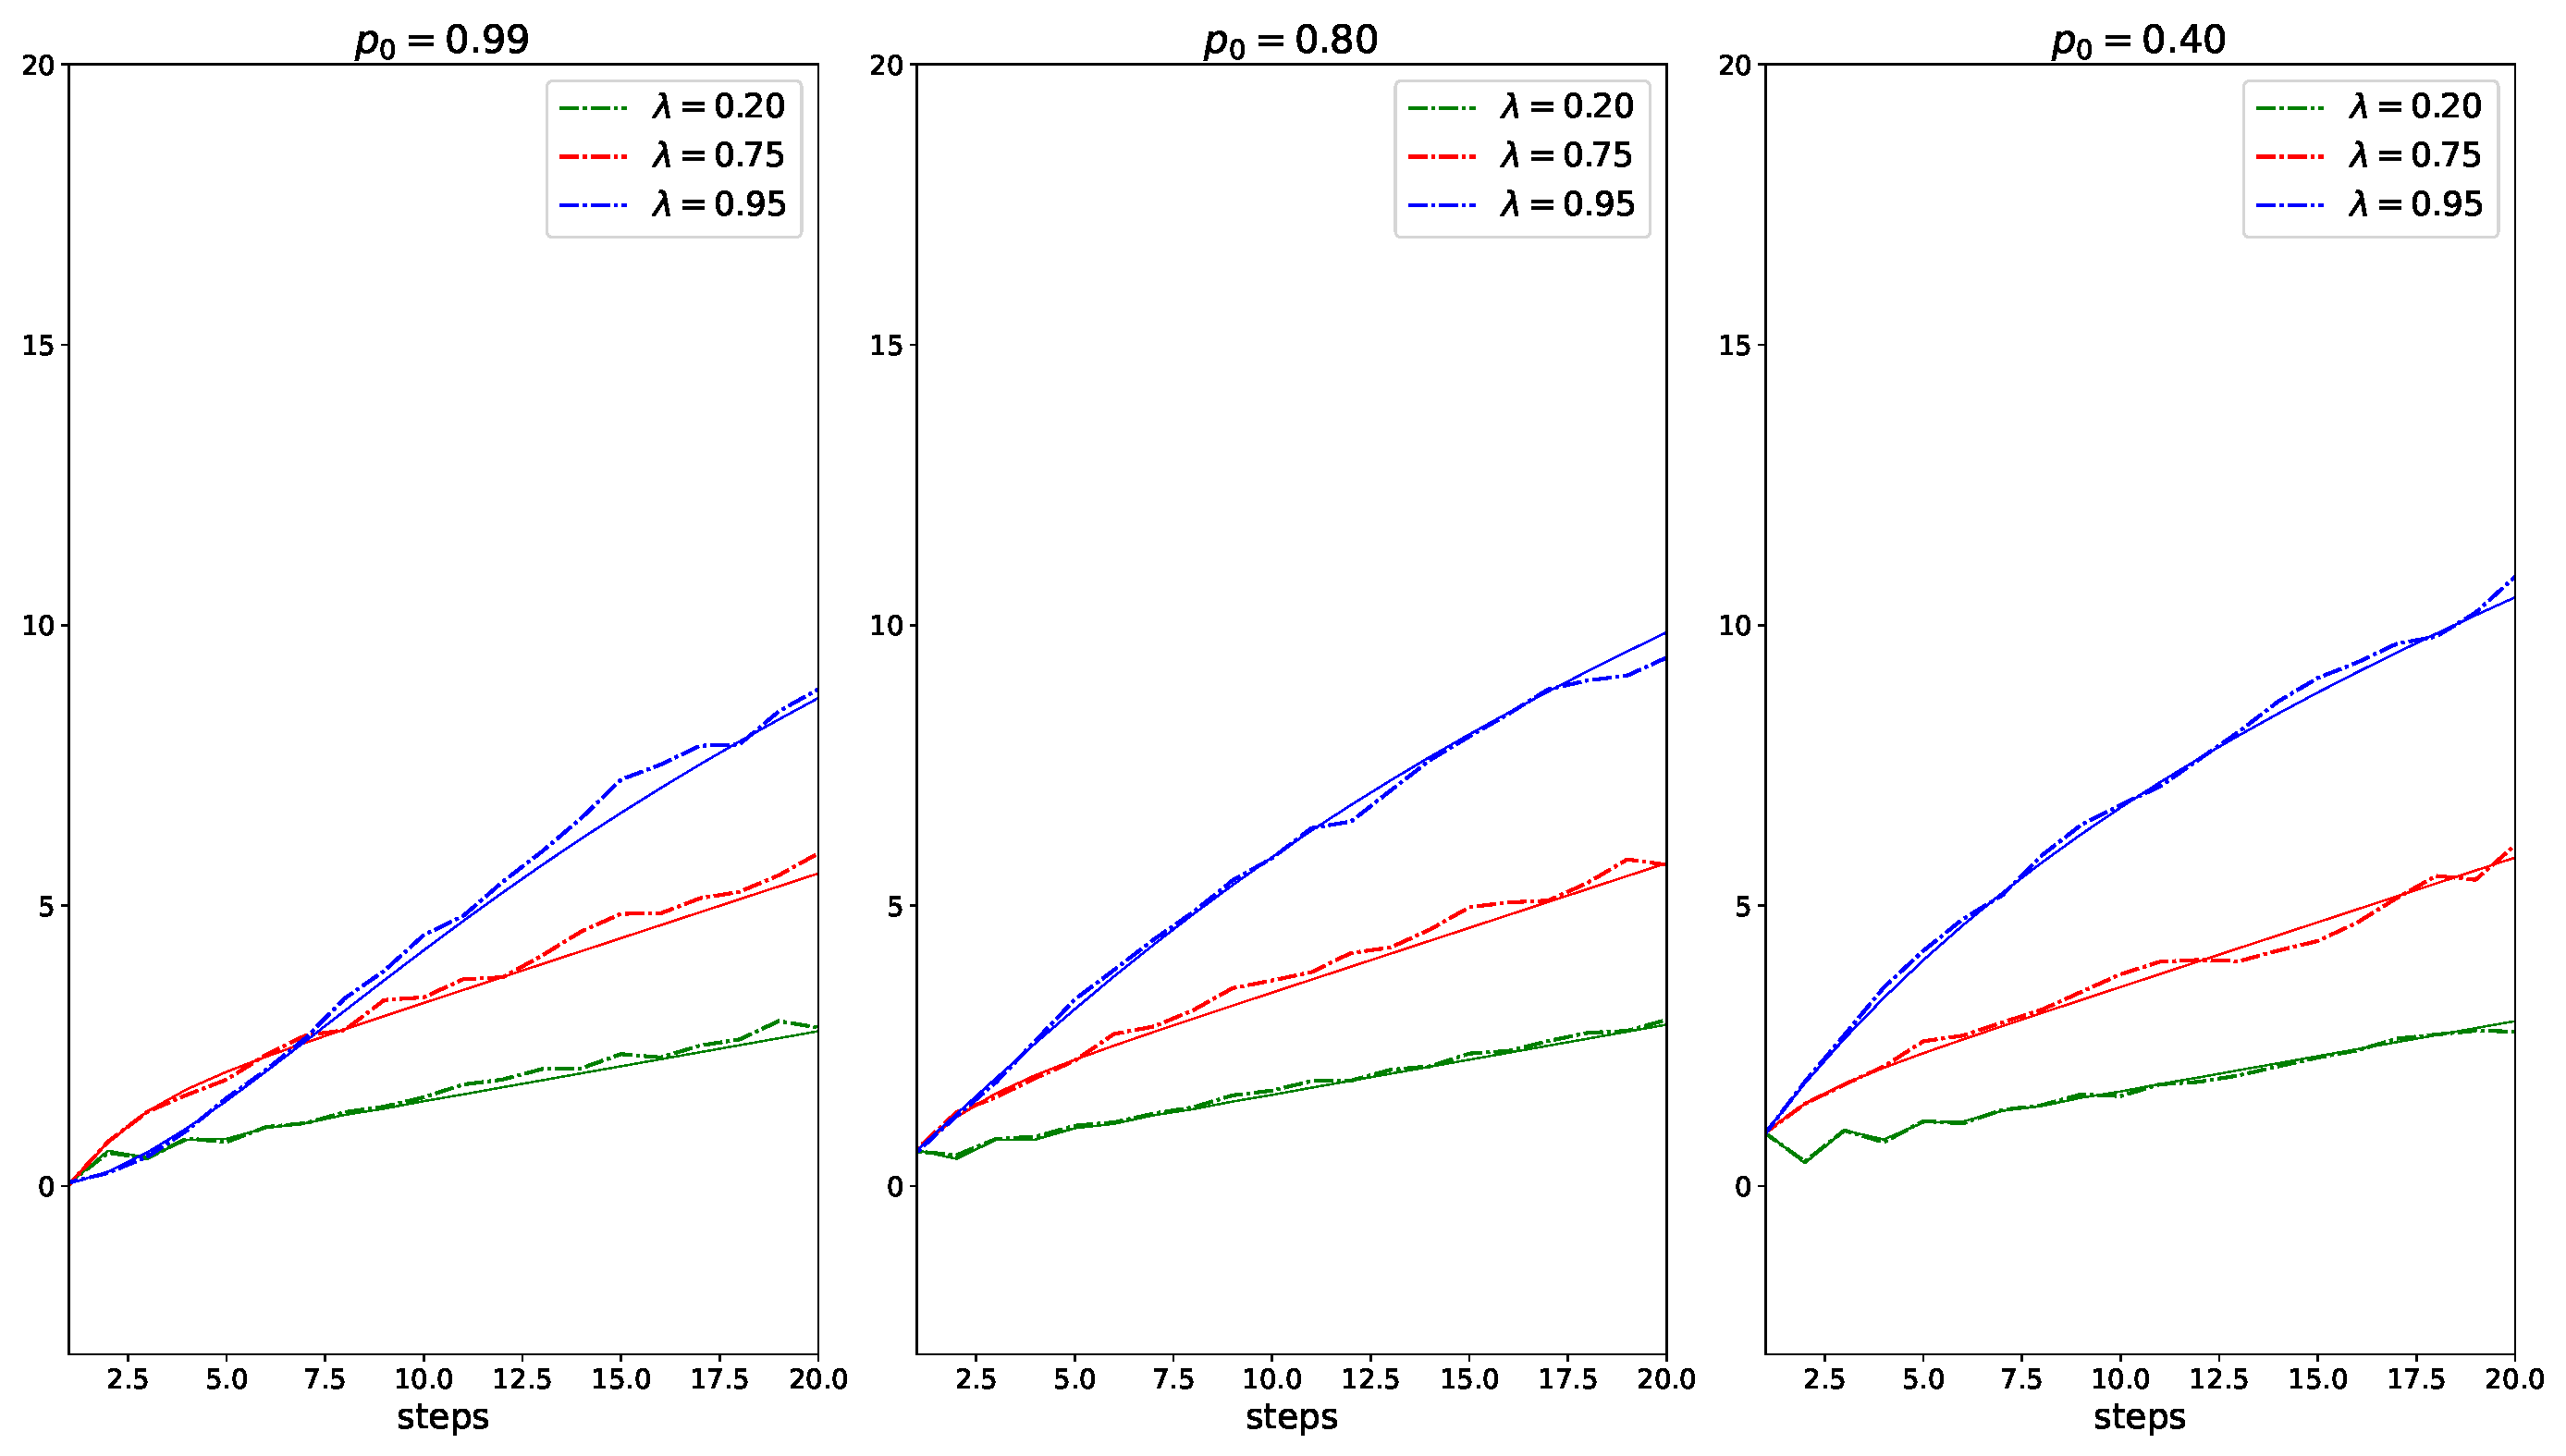
\includegraphics[width=1\textwidth]{../simulations/e_position_1000_walks_20_steps_type_success_punished}

        \caption{\label{fig:var_s_t_sp}Observed (dash-dotted) and theoretical (solid
        lines) values of $Var\,S_{t}$ -- \emph{success punishing }model.
        The
        data were obtained from 1000 walks generated with given parameters. }

    \end{figure}

    \subsection{Success rewarding model}\label{subsec:success-rewarding-model}

    Similar formulas can be derived for the \emph{success rewarding }model.
    Once again for previous results only the formulas are presented with
    proofs in the referred literature, new properties are derived with
    full complexity.
    For the sake of clarity the set of expressions is
    presented in the same manner as in the previous section.

    For the expected value and variance of the step size for the $t\ge1$
    iteration of the walk $X_{t}$ it holds~\cite{ja2019apmat}
    \begin{equation}
        EX_{t}=2p_{0}-1,\label{eq:e_x_t_sr}
    \end{equation}
    \begin{equation}
        Var\,X_{t}=4p_{0}(1-p_{0}).\label{eq:var_x_t_sr}
    \end{equation}

    For the expected value and variance of the transition probability
    for the $t\ge1$ iteration of the walk $P_{t}$ it holds~\cite{ja2019apmat}
    \begin{equation}
        EP_{t}=p_{0},\label{eq:e_p_t_sr}
    \end{equation}
    \begin{equation}
        Var\,P_{t}=(2\lambda-\lambda^{2})^{t}p_{0}^{2}+p_{0}(1-\lambda)^{2}\sum_{i=0}^{t-1}(2\lambda-\lambda^{2})^{i}-p_{0}^{2}.\label{eq:var_p_t_sr}
    \end{equation}
    As the sum in the formula equals $\frac{1-(2\lambda-\lambda^{2})^{t}}{1-(2\lambda-\lambda^{2})}$,
    it can be further simplified as
    \begin{gather*}
        Var\,P_{t}=(2\lambda-\lambda^{2})^{t}p_{0}^{2}+p_{0}(1-\lambda)^{2}\frac{1-(2\lambda-\lambda^{2})^{t}}{(1-\lambda)^{2}}-p_{0}^{2}=\\
        =p_{0}[(2\lambda-\lambda^{2})^{t}(p_{0}-1)+1]-p_{0}^{2},\\
        Var\,P_{t}=p_{0}(1-p_{0})(1-(2\lambda-\lambda^{2})^{t}).\\
    \end{gather*}

    Finally, the expected position of the walker $S_{t}$ after $t\geq1$
    iterations can be expressed as~\cite{ja2019apmat}
    \begin{equation}
        ES_{t}=S_{0}+t(2p_{0}-1).\label{eq:e_s_t_sr}
    \end{equation}

    To prove a formula allowing to compute the variance of the position
    of the walker, let us again start with a support proposition.
    \begin{proposition}
        For all $t\ge1$
        \begin{equation}
            E(P_{t}S_{t})=p_{0}S_{0}+p_{0}t+2\lambda p_{0}(p_{0}-1)\frac{1-(2\lambda-\lambda^{2})^{t}}{(1-\lambda)^{2}}.\label{eq:e_p_s_t_sr}
        \end{equation}
    \end{proposition}

    \begin{proof}
        We will once again start with expressing $E(P_{t}S_{t})$ from the
        knowledge of the past step.
        \begin{gather*}
            E(P_{t}S_{t})=E(E(P_{t-1}S_{t-1}|P_{t-1})=\\
            =E[E((\lambda P_{t-1}+\frac{1}{2}(1-\lambda)(1+X_{t}))(S_{t-1}+X_{t})|P_{t-1})]=\\
            =E[E(\lambda P_{t-1}S_{t-1}+\frac{1-\lambda}{2}S_{t-1}+\frac{1-\lambda}{2}X_{t}S_{t-1}+\\
                +\lambda X_{t}P_{t-1}+\frac{1-\lambda}{2}X_{t}+\frac{1-\lambda}{2}X_{t}^{2}|P_{t-1})]\\
        \end{gather*}
        and using $E(X_{t}|P_{t-1})=2P_{t-1}-1$ and $EX_{t}^{2}=1$ finally
        \begin{equation}
            E(P_{t}S_{t})=E(P_{t-1}S_{t-1})+2\lambda EP_{t-1}^{2}-(2\lambda-1)EP_{t-1}.\label{eq:e_p_s_t-1_t_sr}
        \end{equation}
        Further we will continue using mathematical induction.
        For $t=1$
        using the definition of the walk it holds that
        \begin{gather*}
            E(P_{1}S_{1})=p_{0}(1-(1-p_{0})\lambda)(S_{0}+1)+(1-p_{0})\lambda p_{0}(S_{0}-1)=\\
            =p_{0}S_{0}+2\lambda p_{0}^{2}-(2\lambda-1)p_{0}.\\
        \end{gather*}
        When substituting $t=1$ into~\eqref{eq:e_p_s_t_sr} we obtain
        \begin{gather*}
            E(P_{1}S_{1})=p_{0}S_{0}+p_{0}+2\lambda p_{0}(p_{0}-1)\frac{1-(2\lambda-\lambda^{2})^{0}}{(1-\lambda)^{2}}=\\
            =p_{0}S_{0}+p_{0}+2\lambda p_{0}(p_{0}-1)\\
        \end{gather*}
        and finally
        \[
            E(P_{1}S_{1})=p_{0}S_{0}+2\lambda p_{0}^{2}-(2\lambda-1)p_{0}.
        \]
        Equation~\eqref{eq:e_p_s_t_sr} thus holds for $t=1$.
        Now for the
        induction step $t\rightarrow t+1$ we get by substituting \eqref{eq:e_p_s_t_sr}
        into (\ref{eq:e_p_s_t-1_t_sr})
        \[
            E(P_{t+1}S_{t+1})=E(P_{t}S_{t})+2\lambda EP_{t}^{2}-(2\lambda-1)EP_{t}
        \]
        and further using
        \[
            EP_{t}^{2}=p_{0}((2\lambda-\lambda^{2})^{t}(p_{0}-1)+1),
        \]
        which follows from the proof of Proposition 3.7 in~\cite{ja2019apmat},
        and~\eqref{eq:e_p_t_sr}
        \begin{gather*}
            E(P_{t+1}S_{t+1})=p_{0}S_{0}+p_{0}t+2\lambda p_{0}(p_{0}-1)\frac{1-(2\lambda-\lambda^{2})^{t}}{(1-\lambda)^{2}}+\\
            +2\lambda p_{0}((2\lambda-\lambda^{2})^{t}(p_{0}-1)+1)-(2\lambda-1)p_{0}=\\
            =p_{0}S_{0}+p_{0}(t+1)+2\lambda p_{0}(p_{0}-1)[\frac{1-(2\lambda-\lambda^{2})^{t}}{(1-\lambda)^{2}}+(2\lambda-\lambda^{2})^{t}]=\\
            =p_{0}S_{0}+p_{0}(t+1)+2\lambda p_{0}(p_{0}-1)\frac{1-(2\lambda-\lambda^{2})^{t+1}}{(1-\lambda)^{2}}.\\
        \end{gather*}
    \end{proof}
    \begin{theorem}
        \label{thm:var_s_t_sr}For all $t\ge1$ holds
        \[
            Var\,S_{t}=4p_{0}(1-p_{0})t^{2}+a(p_{0},\lambda)t-a(p_{0},\lambda)\frac{1-(2\lambda-\lambda^{2})^{t}}{(1-\lambda)^{2}},
        \]
        where
        \[
            a(p_{0},\lambda)=\frac{8p_{0}(1-p_{0})}{(1-\lambda)^{2}}.
        \]
    \end{theorem}

    \begin{proof}
        As clearly the value $S_{0}$ does not affect the variance, let us
        from now assume $S_{0}=0$.
        From the definition of variance and~\eqref{eq:e_s_t_sr}
        follows that to prove the theorem it is enough to prove that
        \begin{equation}
            ES_{t}^{2}=t^{2}+a(p_{0},\lambda)t-a(p_{0},\lambda)\frac{1-(2\lambda-\lambda^{2})^{t}}{(1-\lambda)^{2}}.\label{eq:e_s2_t_sr}
        \end{equation}
        First of all let us recall that formula (\ref{eq:e_s2_t-1_t_sp})
        holds for the \emph{success rewarding} type of the model as well.
        The theorem will be once again proved using mathematical induction.
        For $t=1$ the definition of the walk yields the same result as in
        the proof of Theorem~\ref{thm:VarSt_sp}.
        By substituting $t=1$
        into~\eqref{eq:e_s2_t_sr} we obtain
        \[
            ES_{1}^{2}=1+a(p_{0},\lambda)-a(p_{0},\lambda)=1
        \]
        and~\eqref{eq:e_s2_t_sr} thus holds for $t=1$.
        Now for the induction
        step $t\rightarrow t+1$ we get by substituting~\eqref{eq:e_s2_t_sr},~\eqref{eq:e_p_s_t_sr} and~\eqref{eq:e_s_t_sr} into (\ref{eq:e_s2_t-1_t_sp})
        \begin{gather*}
            ES_{t+1}^{2}=ES_{t}^{2}+4E(P_{t}S_{t})-2ES_{t}+1=\\
            =t^{2}+a(p_{0},\lambda)t-a(p_{0},\lambda)\frac{1-(2\lambda-\lambda^{2})^{t}}{(1-\lambda)^{2}}+\\
            +4(p_{0}t+2\lambda p_{0}(p_{0}-1)\frac{1-(2\lambda-\lambda^{2})^{t}}{(1-\lambda)^{2}})-2t(2p_{0}-1)+1=\\
            =(t+1)^{2}+a(p_{0},\lambda)(t+1)-a(p_{0},\lambda)\frac{1-(2\lambda-\lambda^{2})^{t+1}}{(1-\lambda)^{2}}.\\
        \end{gather*}
        Substituting~\eqref{eq:e_s2_t_sr} and~\eqref{eq:e_s_t_sr} into the
        definition of variance then proves the theorem.
    \end{proof}
    \begin{corollary}
        \label{cor:var_s_t_sr}For $t\rightarrow+\infty$
        \[
            \lim_{t\rightarrow+\infty}Var\,S_{t}=+\infty
        \]
        and
        \[
            \lim_{t\rightarrow+\infty}\left(Var\,S_{t}-\left(4p_{0}(1-p_{0})t^{2}+a(p_{0},\lambda)t-\frac{a(p_{0,}\lambda)}{(1-\lambda)^{2}}\right)\right)=0,
        \]
        with $a(p_{0},\lambda)$ as in Theorem~\ref{thm:var_s_t_sr}.
    \end{corollary}

    Corollary~\ref{cor:var_s_t_sr} shows that with $t\rightarrow+\infty$
    $Var\,S_{t}$ behaves as a quadratic function with respect to $t$.
    Similarly as with the \emph{success punishing} model, such behavior
    is illustrated on Figure \ref{fig:var_s_t_sr}, which also shows
    the comparision of the theoretical value of position variance and
    an empirical one obtained using simulated data.

    \begin{figure}
        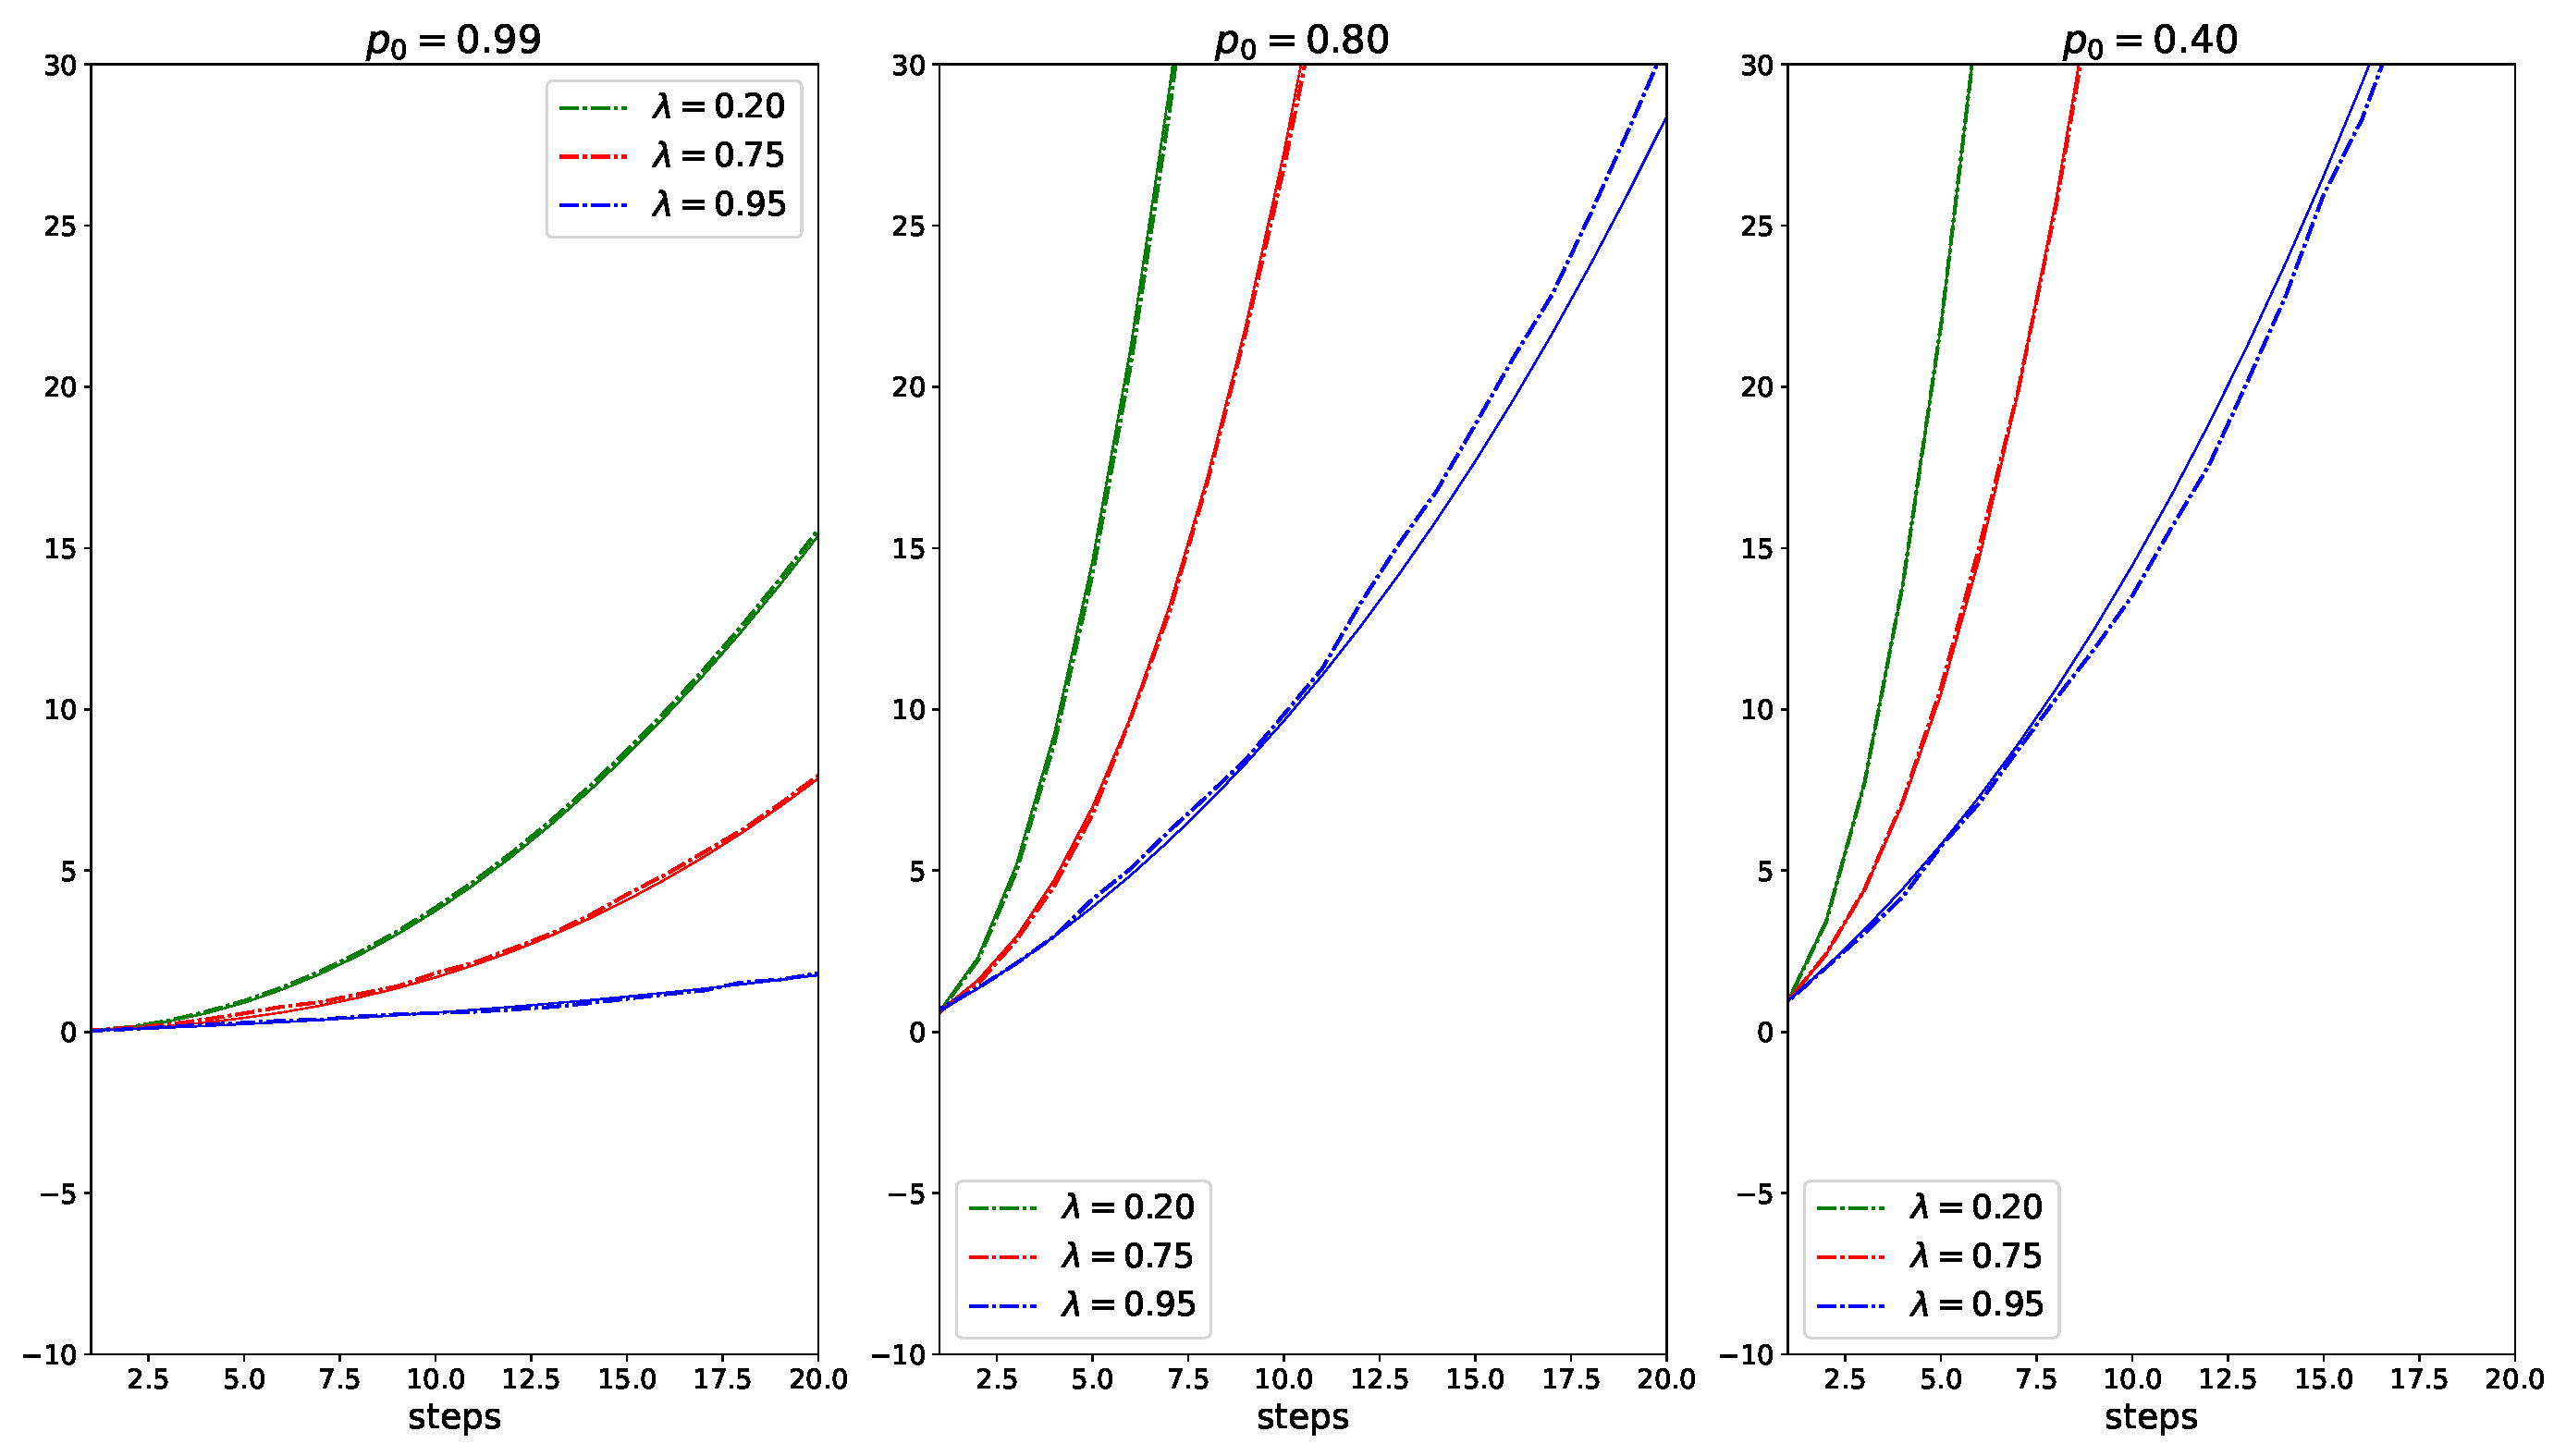
\includegraphics[width=1\textwidth]{../simulations/e_position_1000_walks_20_steps_type_success_rewarded}

        \caption{\label{fig:var_s_t_sr}Observed (dash-dotted) and theoretical (solid
        lines) values of $Var\,S_{t}$ -- \emph{success rewarding }model.
        The
        data were obtained from 1000 walks generated with given parameters. }

    \end{figure}

    \subsection{Two-parameter models}\label{subsec:two-parameter-models}

    The presented model can be further extended by adding additional levels
    of complexity.
    The first option is to use two separate $\lambda$
    parameters for each direction of the walk.
    Maintaining the two basic
    options -- \emph{success punishing} and \emph{success rewarding} models --
    this level of complexity can defined as follows~\cite{ja2019apmat}.
    \begin{definition}
        Let $\ensuremath{p_{0},\lambda_{0},\lambda_{1}\in(0,\,1)}$ be constant
        parameters, ${\{P_{n}\}}_{n=0}^{\infty}$ and ${\{X_{n}\}}_{n=1}^{\infty}$
        sequences of discrete random variables with $P_{0}=p_{0}$.
        For $t\ge1$ let
        \[
            P(X_{t}=1|P_{t-1}=p_{t-1})=p_{t-1},\,\,\,P(X_{t}=-1|P_{t-1}=p_{t-1})=1-p_{t-1},
        \]
        and (\emph{success punishing)}
        \begin{equation}
            P_{t}=\frac{1}{2}[(1+X_{t})\lambda_{0}P_{t-1}+(1-X_{t})(1-\lambda_{1}(1-P_{t-1}))]\label{eq:def_2l_p_sp}
        \end{equation}
        or (\emph{success rewarding)}
        \begin{equation}
            P_{t}=\frac{1}{2}[(1-X_{t})\lambda_{0}P_{t-1}+(1+X_{t})(1-\lambda_{1}(1-P_{t-1}))].\label{eq:def_2l_p_sr}
        \end{equation}
        The sequence ${\{S_{n}\}}{}_{n=0}^{\infty},\;S_{N}=S_{0}+\sum_{i=1}^{N}X_{i}$
        for $n\in\mathbb{N}$, with $S_{0}\in\mathbb{R}$ some given starting
        position, is called a \emph{random walk with varying probabilities
        -- two-parameter model}, with ${\{X_{n}\}}_{n=1}^{\infty}$ being the
        steps of the walker and ${\{P_{n}\}}_{n=0}^{\infty}$ transition probabilities.
        Depending on the chosen formula to calculate $P_{t}$ the walk type
        is either \emph{success punishing}~\eqref{eq:def_2l_p_sp} or \emph{success
        rewarding}~\eqref{eq:def_2l_p_sr}.

        The derivation of exact model properties is not so straightforward
        as in the case with single lambda.
        The properties were thus studied
        with the help of simulations.
        Figures~\ref{fig:var_s_t_2l_sp} and~\ref{fig:var_s_t_2l_sr} present again the variance of $S_{t}$.
        It seems that the position variance of the \emph{success punishing}
        model goes to infinity linearly and of the \emph{success rewarding}
        model quadratically, similarly as in the corresponding single parameter
        scenarios.

        \begin{figure}
            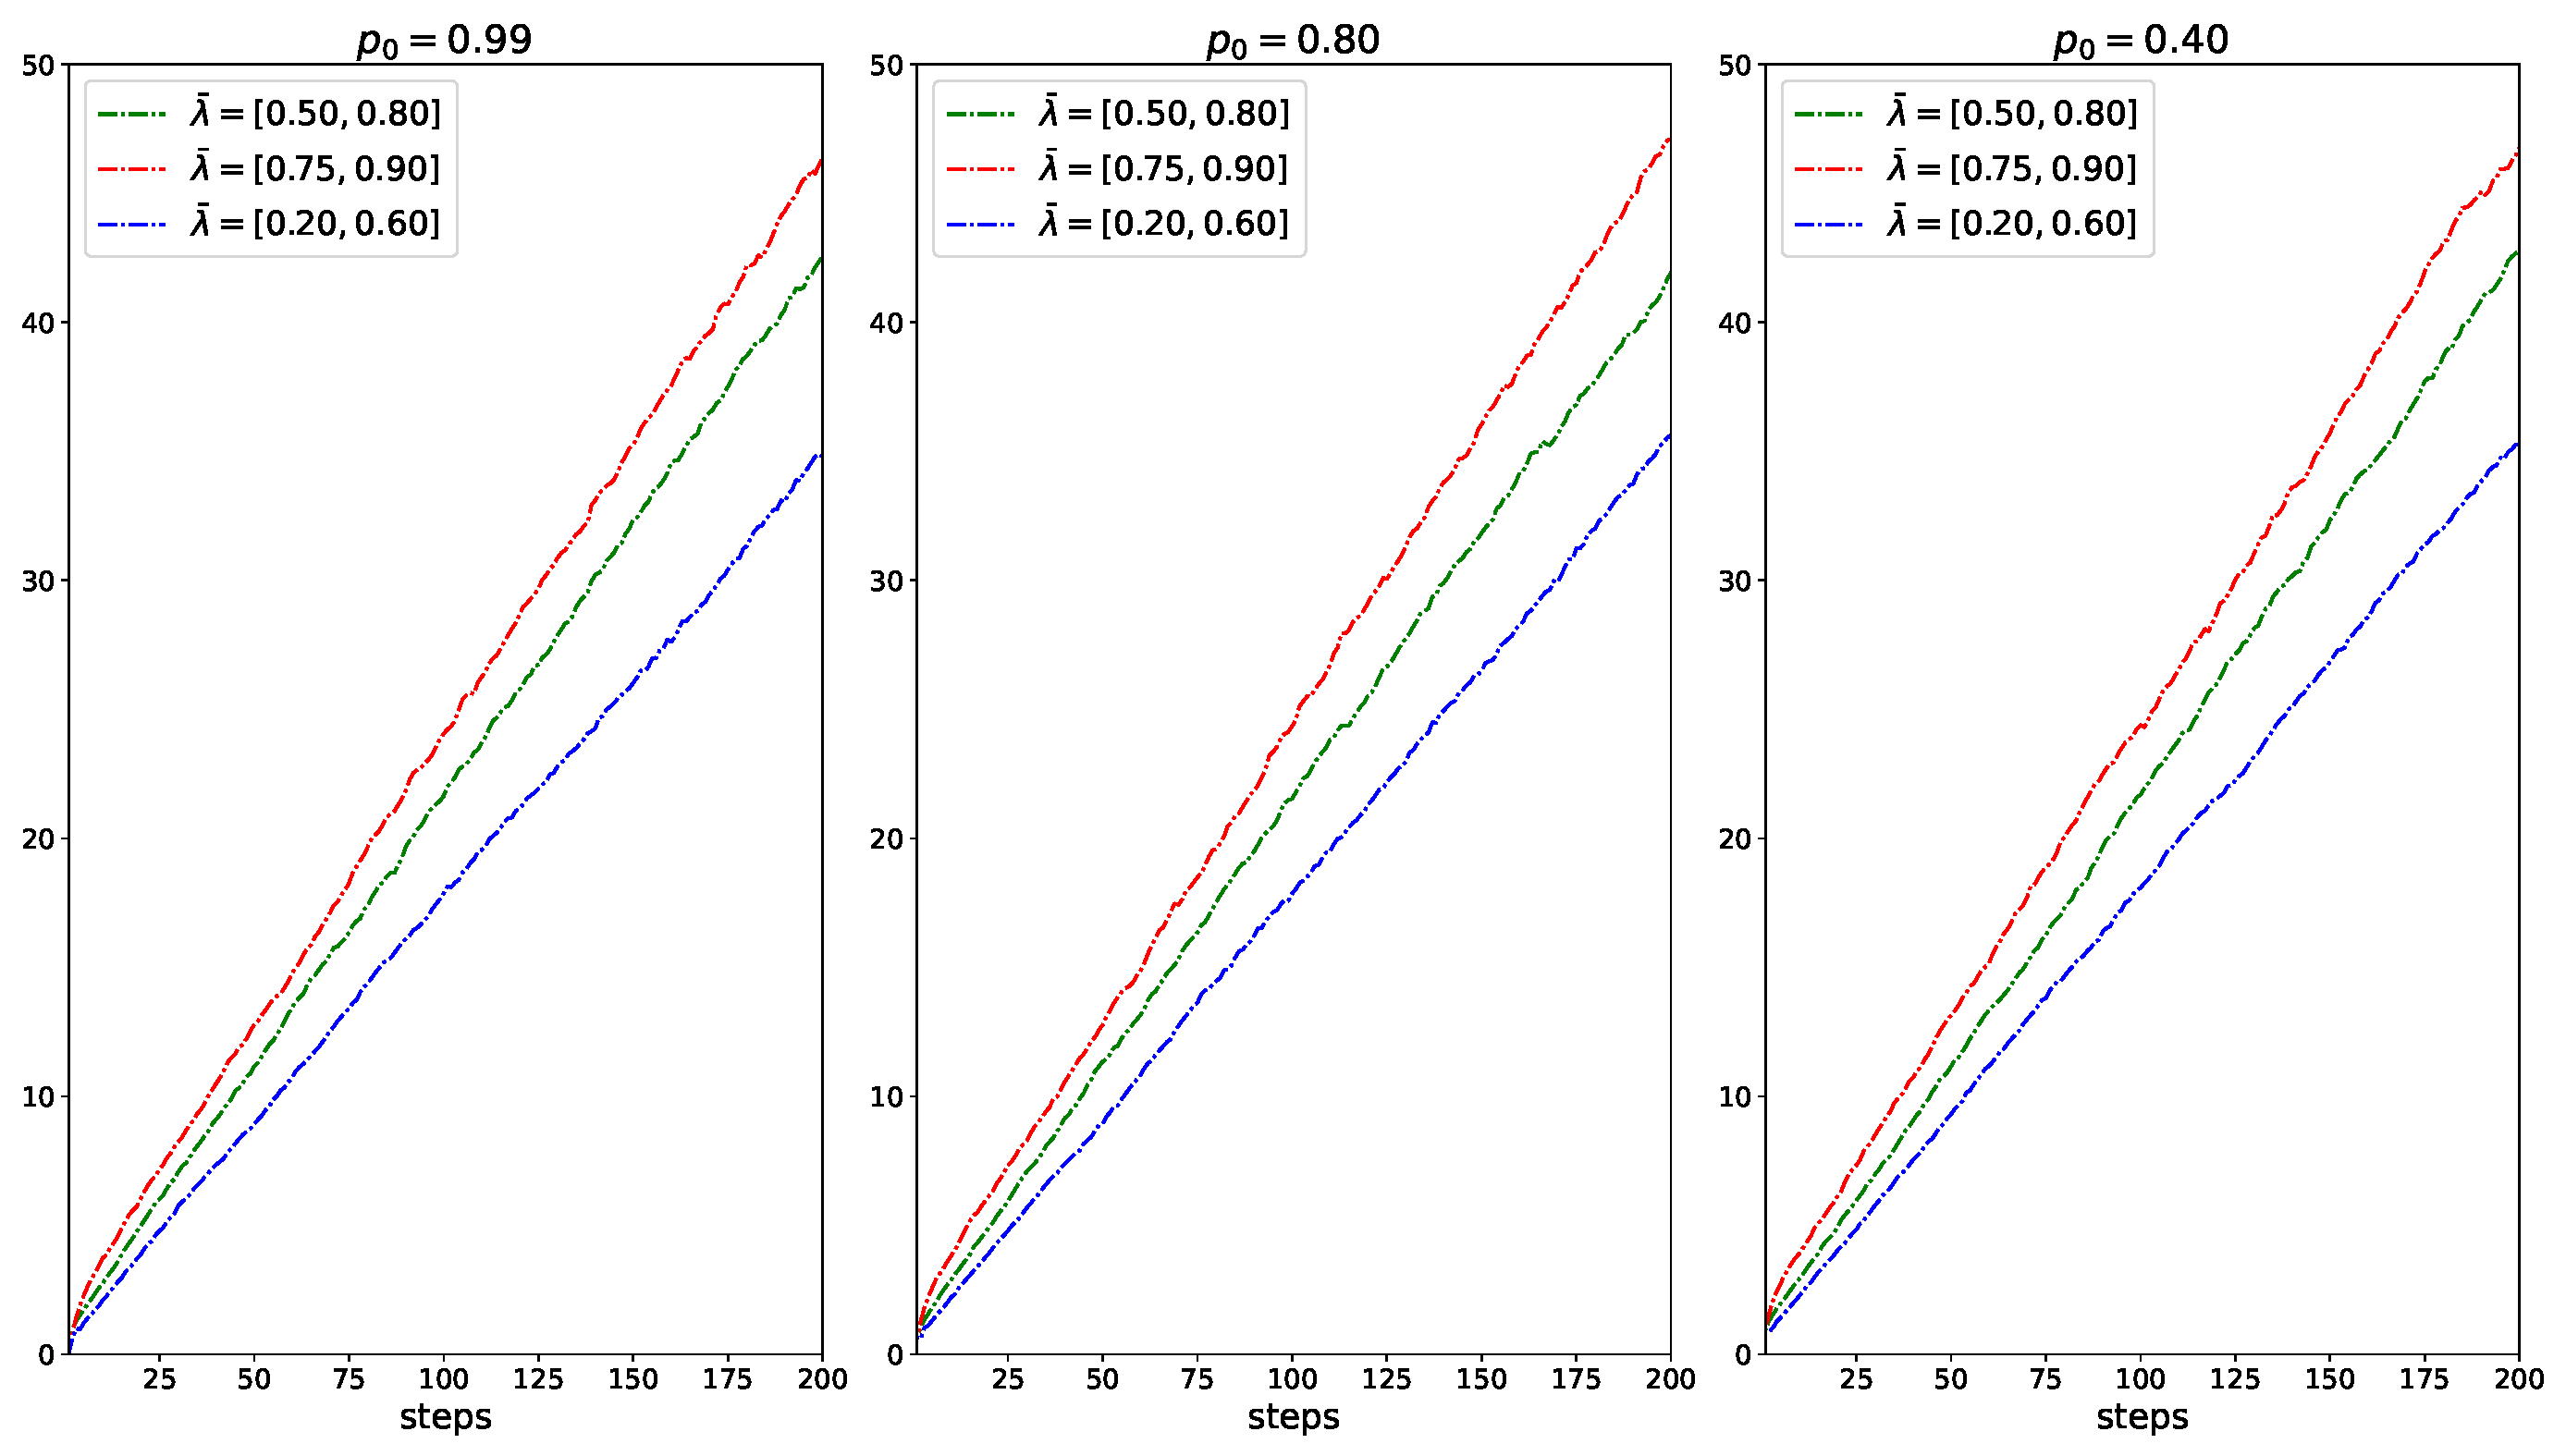
\includegraphics[width=1\textwidth]{../simulations/e_position_10000_walks_200_steps_type_success_punished_two_lambdas}
            \caption{\label{fig:var_s_t_2l_sp}The observed position variance of the \emph{two-parameter
            success punishing} model.
            The data were gathered from $10000$ simulations
            with given parameters.}

        \end{figure}

        \begin{figure}
            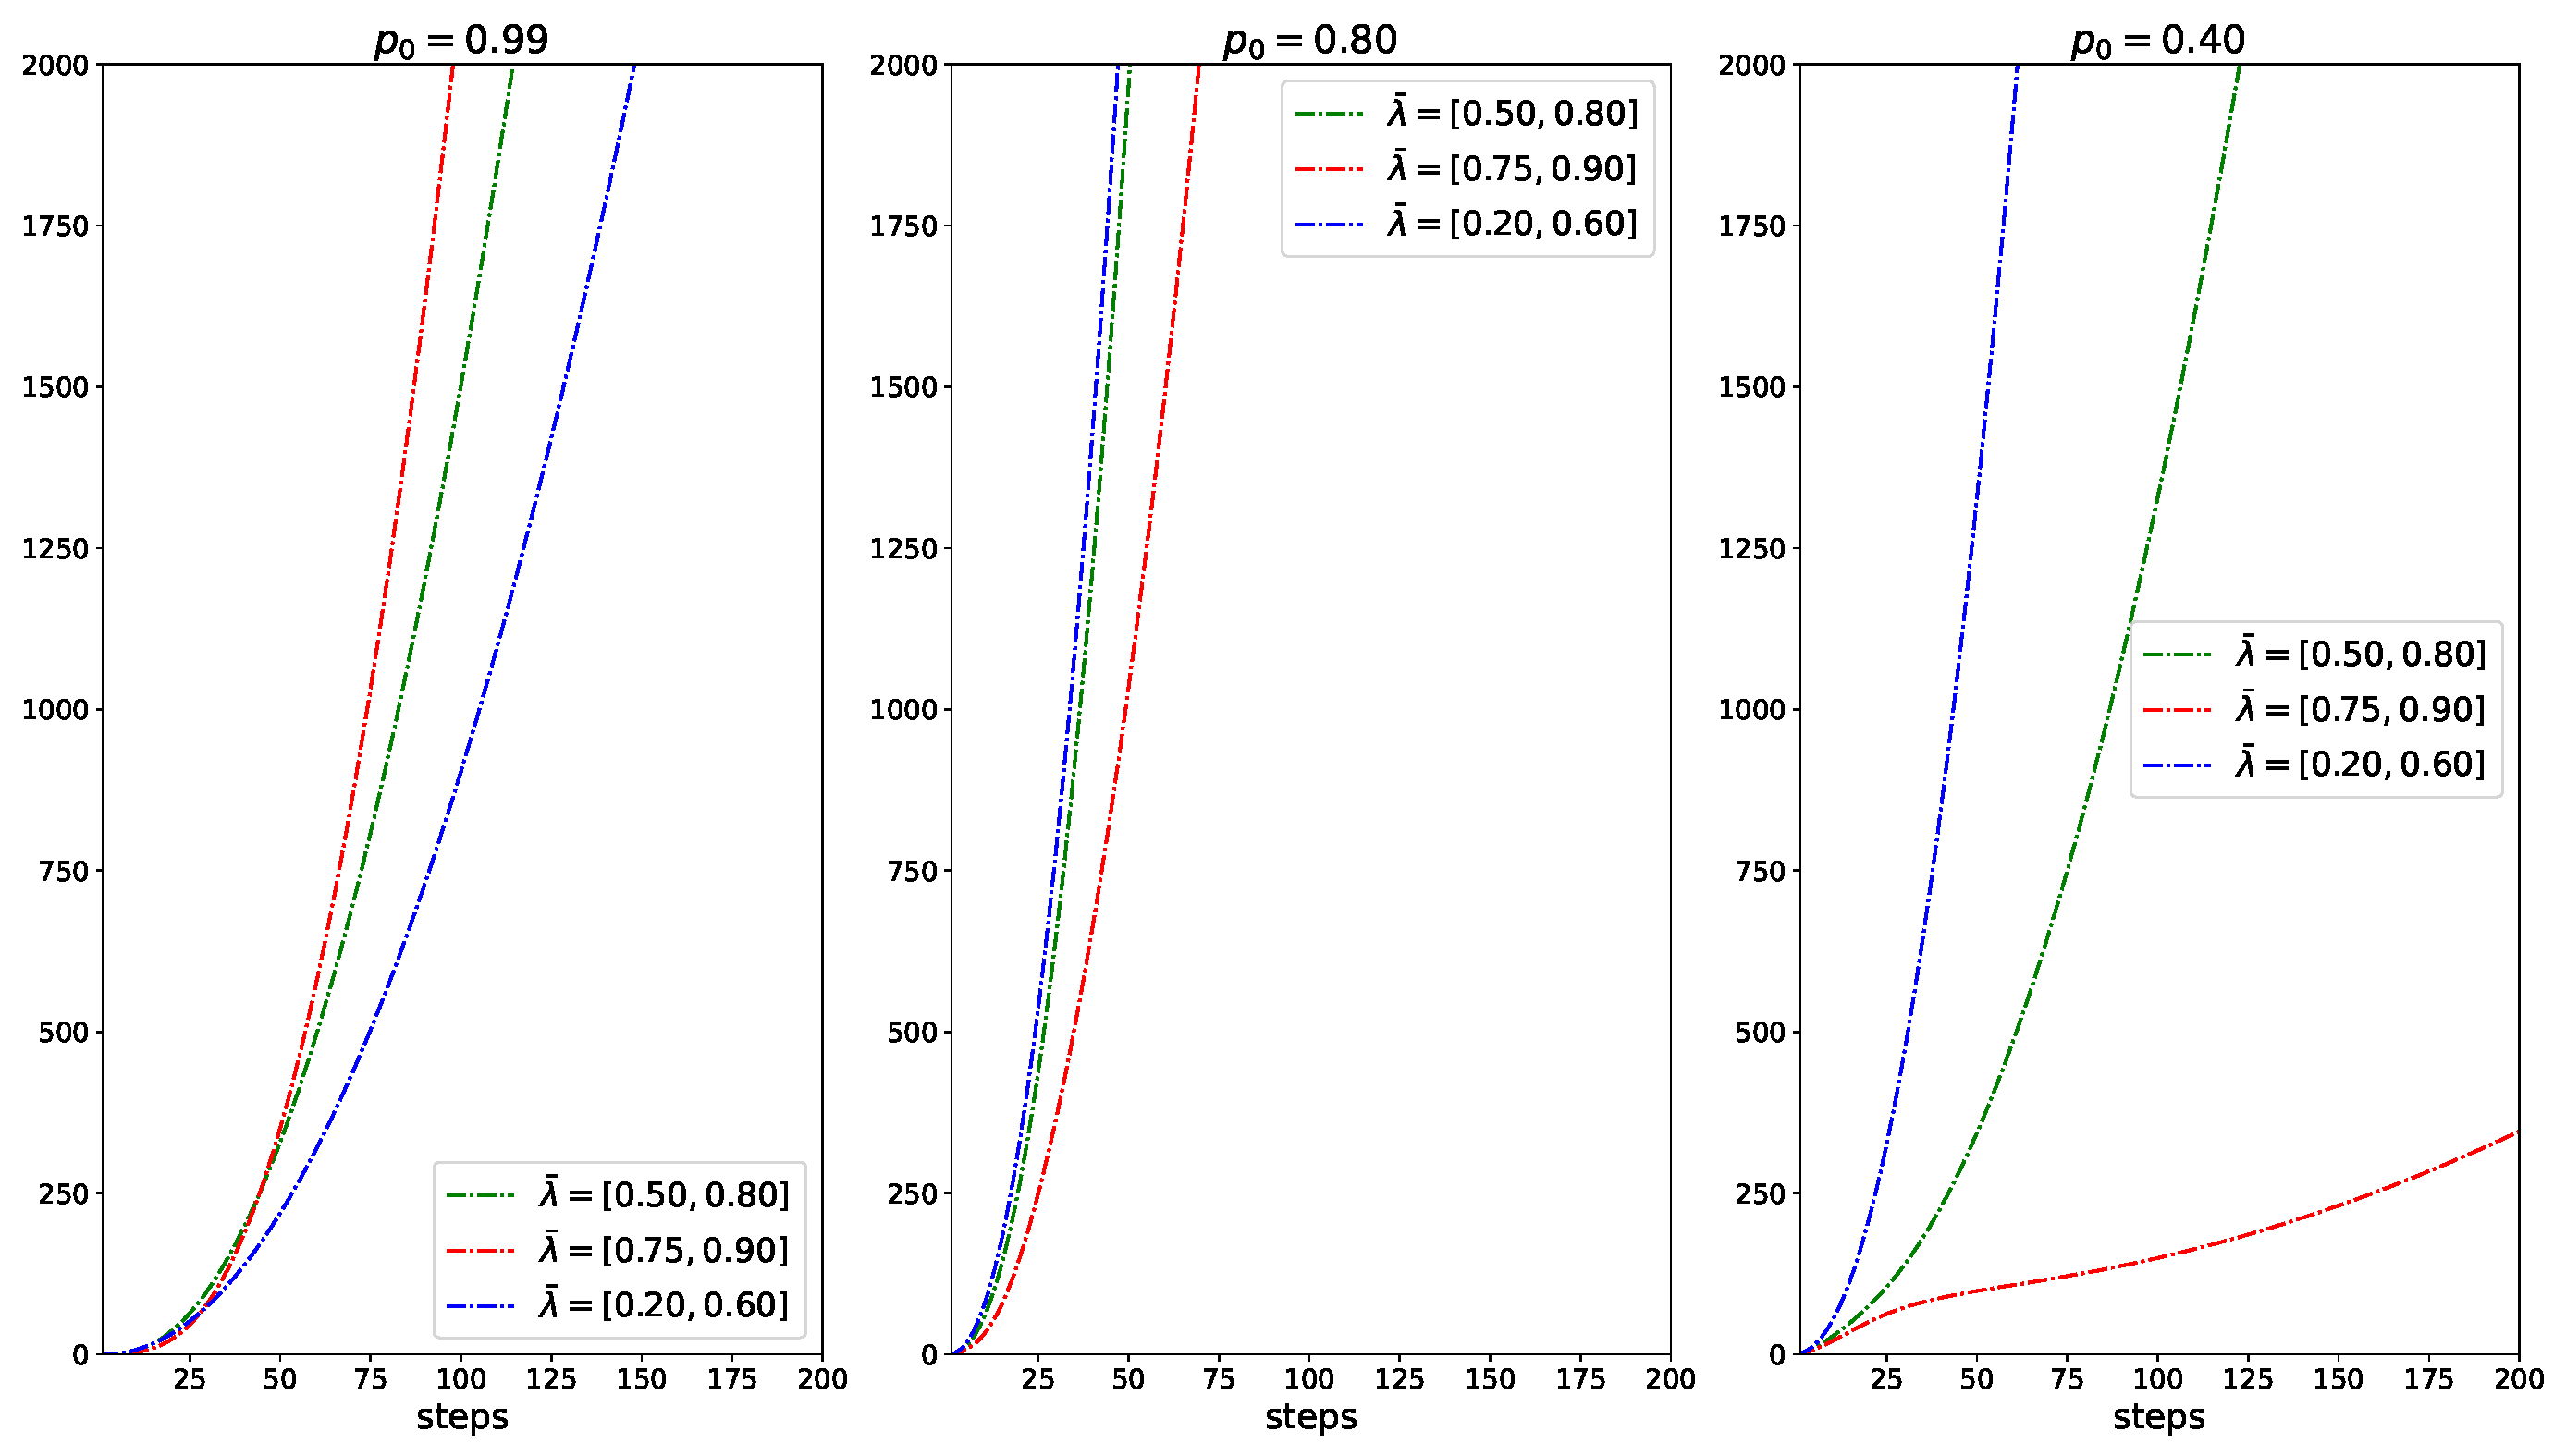
\includegraphics[width=1\textwidth]{../simulations/e_position_10000_walks_200_steps_type_success_rewarded_two_lambdas}

            \caption{\label{fig:var_s_t_2l_sr}The observed position variance of the \emph{two-parameter
            success rewarding} model.
            The data were gathered from $10000$ simulations
            with given parameters.}

        \end{figure}
    \end{definition}

    \subsection{Other model alternatives}\label{subsec:other-model-alternatives}

    There are many possibilities how to further enhance the model.
    The model can be combined with a varying step size model from~\cite{turban2010random},
    the $\lambda$ parameter can be handled as a function of time and position,
    or a combination of varying probability model with regression
    part (e.g. logistic) can be considered, which seems especially promising from application point of view.
    These variations of the model will be subject of further study.


    \section{Model application}\label{sec:Model-application}

    The model is especially well suited for simulation of random processes where a single or just a few events significantly affect the process's future development.
    An example such a process can be found in sports modelling.
    In such applications rather short walks occur, but they can be observed repetitively.
    For example in modelling tennis sets, the longest walk has only 5 steps (occurring in men Grand Slam or Davis Cup matches), but there are many matches played each year,
    which can be (under some assumptions) considered as multiple observations of the same walk.
    The authors recently presented a study where the model was used for modelling the men tennis Grand Slam matches with results suggesting the model might provide precious insights when modelling tennis.
    Here is a brief summary of the modelling approach.

    The \emph{success rewarding} version of the model was selected as the historical results show that the development of a tennis match follows such pattern.
    The $p_{0}$ parameter was obtained using input bookmaker odds from \emph{Pinnacle Sports}, an industry leading bookmaker.
    The appropriate $\lambda$ parameter was then found from historical data using the maximal likelihood estimate.
    The model was tested on a database consisting of $4255$ tennis matches that took place between 2009 and 2018 and the results suggest that such a model could be used for \emph{in-play} odds prediction.
    For full details of the model derivation and testing, see the original paper~\cite{ja2019mathsport_proc}.

    The quality of such \emph{in-play} predictions was tested on a small study in real life setting with active betting against a bookmaker.
    The model from ~\cite{ja2019mathsport_proc} was implemented into an automatic odds scraping and betting tool.
    Whenever the odds provided by bookmaker $a_{i}$  were higher than the model implied odds, i.e. $a_{i}>\frac{1}{p}$, a bet was made.
    This test was carried over the $2019$ men tennis US~Open and resulted in $128$ placed bets with the total amount $59.85$ units bet.
    As the bets were not placed simultaneously, but rather consecutively, the theoretical total bankroll needed for the betting was only $0.52$ units -- the minimal actual account balance over the entire US Open.
    The actual number of wins was $57$, slightly below the number of expected wins, but thanks to the average winning odds of $2.3$ the final balance was plus $2.24$ units,
    creating a theoretical win $\frac{2.24}{0.52}=4.3$ times the investment, which is an outstanding performance.

    This study just briefly shows the possibilities of the presented model and presents rather encouraging results.
    The testing dataset, consisting of only 128 bets, is however too small to provide a strong evidence favoring the model over bookmaker's odds.
    A more conclusive test on a bigger dataset will be subject of further study.


    \section{Conclusion}\label{sec:conclusion}

    The present paper continues in the research on one specific set of
    models of Bernoulli-like random walks, the models where the transition
    probabilities depend on the walk history.
    After reviewing basic models
    types and the results of previous studies, new
    properties of the model characterizing the variability of the walk were proved.
    These properties were explored additionally with the aid
    of simulations in order to compare derived theoretical results with
    empirical ones based on simulated data.
    The problem of parameter
    estimation was not addressed here, the properties of the maximum likelihood
    estimate of both $\lambda$ and $p_{0}$ were studied in depth in~\cite{ja2019apmat} and utilized in~\cite{ja2019mathsport_proc},
    a study devoted to one of possible model applications, namely the
    modelling of tennis matches development.
    This kind of application was briefly recalled also in the present contribution and aggregated results of model testing on a new small dataset were reported.

    \paragraph{Acknowledgement.}
    The research was supported by the grant No. 18--02739S of the Grant Agency of the Czech Republic.


    \bibliographystyle{plain}
    \bibliography{doktknih}

\end{document}
